\documentclass[11pt,a4paper]{article}
\usepackage[utf8]{inputenc}
\usepackage[T1]{fontenc}
\usepackage[sc]{mathpazo}
\usepackage[scaled=0.92]{helvet}
\usepackage{microtype}
\usepackage[a4paper,top=2.6cm,bottom=2.4cm,left=2.4cm,right=2.4cm,headheight=14pt]{geometry}
\usepackage[table]{xcolor}
\usepackage{booktabs,array,enumitem,multirow}
\usepackage{tikz}
\usetikzlibrary{calc,positioning}
\usepackage{pgfplots}
\pgfplotsset{compat=1.16}
\usepackage[most]{tcolorbox}
\usepackage{titlesec}
\usepackage{needspace,etoolbox}
\usepackage{fancyhdr}
\usepackage{caption}
\usepackage{url}
\def\UrlBreaks{\do\/\do\-\do\_\do\.\do\=\do\?\do\&\do\a\do\b\do\c\do\d\do\e\do\f\do\g\do\h\do\i\do\j\do\k\do\l\do\m\do\n\do\o\do\p\do\q\do\r\do\s\do\t\do\u\do\v\do\w\do\x\do\y\do\z}
\Urlmuskip=0mu plus 1mu
\urlstyle{same}
\usepackage[hidelinks]{hyperref}

% ---- Palet (selaras dengan halaman dokumen pelengkap) ----
\definecolor{teal}{HTML}{0A6C6E}
\definecolor{tealdark}{HTML}{07484A}
\definecolor{ink}{HTML}{13262A}
\definecolor{muted}{HTML}{51666A}
\definecolor{rule}{HTML}{D3DEDC}
\definecolor{pale}{HTML}{EEF5F4}
\definecolor{amber}{HTML}{B7791F}
\definecolor{amberpale}{HTML}{FBF4E4}
\definecolor{well}{HTML}{CFE3E0}

\renewcommand{\tablename}{Tabel}
\renewcommand{\figurename}{Gambar}
\renewcommand{\refname}{Daftar Pustaka}
\color{ink}
\setlength{\parindent}{0pt}
\setlength{\parskip}{6.5pt plus 1pt}
\linespread{1.06}
\tolerance=1200
\emergencystretch=3em
\hyphenpenalty=1500
\setlist{itemsep=2.5pt,topsep=3pt,parsep=0pt,leftmargin=1.4em}
\setlist[itemize]{label={\color{teal}\textbullet}}
\renewcommand{\arraystretch}{1.22}
\setlength{\tabcolsep}{5pt}
\captionsetup{font={small,sf,color=muted},labelfont={bf,color=teal},labelsep=period,justification=raggedright,singlelinecheck=false,skip=5pt}

% ---- Judul bagian ----
\titleformat{\section}{\sffamily\bfseries\Large\color{ink}}{\color{teal}\thesection}{0.7em}{}[{\color{rule}\titlerule[0.6pt]}]
\titlespacing*{\section}{0pt}{18pt}{9pt}
\titleformat{\subsection}{\sffamily\bfseries\normalsize\color{tealdark}}{\color{teal}\thesubsection}{0.6em}{}
\titlespacing*{\subsection}{0pt}{11pt}{3pt}

% ---- Kepala dan kaki halaman ----
\pagestyle{fancy}
\fancyhf{}
\renewcommand{\headrulewidth}{0pt}
\fancyhead[L]{\sffamily\scriptsize\color{muted}\textsc{Alergen}\ \raisebox{0.15ex}{\tiny$\bullet$}\ Dokumen Produksi}
\fancyhead[R]{\sffamily\scriptsize\color{muted}Kit Diagnostik Alergi Berbasis Patch}
\fancyfoot[L]{\sffamily\scriptsize\color{muted}Universitas Airlangga \ $\cdot$ \ IDS000011522}
\fancyfoot[R]{\sffamily\small\bfseries\color{teal}\thepage}
\renewcommand{\headrule}{\color{rule}\hrule width\headwidth height 0.5pt}
\renewcommand{\headrulewidth}{0.5pt}
\fancypagestyle{plain}{\fancyhf{}\renewcommand{\headrulewidth}{0pt}\fancyfoot[R]{\sffamily\small\bfseries\color{teal}\thepage}}

% ---- Tabel ----
\newcommand{\tH}[1]{\textcolor{white}{\sffamily\bfseries\small #1}}
\newcommand{\tabstart}{\small\rowcolors{2}{white}{pale}\arrayrulecolor{rule}}
\newcommand{\hdrrow}{\rowcolor{tealdark}}
\newcolumntype{L}[1]{>{\raggedright\arraybackslash}p{#1}}
\newcolumntype{R}[1]{>{\raggedleft\arraybackslash}p{#1}}
\setlength{\aboverulesep}{0pt}\setlength{\belowrulesep}{0pt}
\renewcommand{\toprule}{\arrayrulecolor{tealdark}\specialrule{0.9pt}{0pt}{0pt}\arrayrulecolor{rule}}
\renewcommand{\bottomrule}{\arrayrulecolor{tealdark}\specialrule{0.9pt}{0pt}{0pt}\arrayrulecolor{rule}}

% ---- Kotak catatan dan kartu angka ----
\newtcolorbox{catatan}[1][Catatan]{enhanced,breakable,colback=amberpale,colframe=amberpale,boxrule=0pt,
  borderline west={2.2pt}{0pt}{amber},arc=1.5pt,left=10pt,right=8pt,top=6pt,bottom=6pt,
  before skip=8pt,after skip=10pt,
  title={\sffamily\bfseries\small\color{amber}\MakeUppercase{#1}},coltitle=amber,
  attach boxed title to top left={yshift=-2mm,xshift=0pt},boxed title style={empty,left=0pt,top=0pt,bottom=0pt},
  fonttitle=\sffamily,coltext=ink,before upper={\vspace{2pt}}}
\newtcolorbox{kartu}[2]{enhanced,colback=pale,colframe=pale,boxrule=0pt,arc=3pt,
  left=8pt,right=6pt,top=6pt,bottom=6pt,halign=left,
  borderline west={2.5pt}{0pt}{teal},
  before upper={{\sffamily\bfseries\LARGE\color{teal}#1}\par\vspace{1pt}},
  fontupper=\sffamily\scriptsize\color{muted},height=1.95cm,valign=top}
\newcommand{\kartuRow}[4]{%
 \begin{tcbraster}[raster columns=#1,raster equal height,raster column skip=7pt,raster row skip=7pt]#2#3#4\end{tcbraster}\vspace{9pt}}

% ---- Sampul ----
\newcommand{\patchmotif}[2]{% #1 skala, #2 warna garis
 \begin{scope}[scale=#1]
 \draw[#2,line width=1.2pt,rounded corners=9pt] (0,0) rectangle (15,6);
 \foreach \r in {0,1}{\foreach \c in {0,...,4}{
   \draw[#2,line width=1pt] ({1.9+\c*2.7},{4.1-\r*2.2}) circle (0.9);}}
 \end{scope}}

\newcommand{\makecover}[5]{% kode, judul, subjudul, tagline, ringkasan satu kalimat
\begin{titlepage}
\thispagestyle{empty}
\begin{tikzpicture}[remember picture,overlay]
 \fill[tealdark] (current page.north west) rectangle ($(current page.north east)+(0,-17.2cm)$);
 \fill[teal!85!tealdark] ($(current page.north east)+(0,-17.2cm)$) -- ($(current page.north east)+(-10cm,-17.2cm)$) -- ($(current page.north east)+(0,-10.8cm)$) -- cycle;
 \begin{scope}[shift={($(current page.north east)+(-9.9cm,-6.4cm)$)}]
   \patchmotif{0.5}{white!35}
 \end{scope}
 \node[anchor=north west,text=white!70,font=\sffamily\small\bfseries,align=left] at ($(current page.north west)+(2.4cm,-2.7cm)$) {\textsc{Alergen \ $\cdot$ \ Universitas Airlangga}};
 \node[anchor=north west,text=white,font=\sffamily\bfseries\fontsize{44}{44}\selectfont] at ($(current page.north west)+(2.4cm,-7.4cm)$) {#1};
 \node[anchor=north west,text=white,font=\sffamily\bfseries\fontsize{26}{31}\selectfont,text width=14.2cm,align=left] at ($(current page.north west)+(2.4cm,-10.2cm)$) {#2};
 \node[anchor=north west,text=white!85,font=\sffamily\fontsize{13}{17}\selectfont,text width=14cm,align=left] at ($(current page.north west)+(2.4cm,-14.1cm)$) {\hyphenpenalty=10000\exhyphenpenalty=10000 #3};
 \node[anchor=north west,text=ink,font=\fontsize{12}{17}\selectfont,text width=15.2cm,align=left] at ($(current page.north west)+(2.4cm,-18.8cm)$) {#4};
 \draw[teal,line width=2pt] ($(current page.north west)+(2.4cm,-21.9cm)$) -- ++(2.2cm,0);
 \node[anchor=north west,text=muted,font=\sffamily\small,text width=15cm,align=left] at ($(current page.north west)+(2.4cm,-22.4cm)$) {%
  \textbf{\color{ink}Kit Diagnostik Alergi Berbasis Patch (Alergen)}\\[3pt]
  Universitas Airlangga, Surabaya\\
  Paten Sederhana IDS000011522\\
  Oktober 2026};
 \node[anchor=south east,text=muted,font=\sffamily\scriptsize,align=right] at ($(current page.south east)+(-2.4cm,1.6cm)$) {#5};
\end{tikzpicture}
\end{titlepage}
\newpage}

\definecolor{sr1}{HTML}{8AA6AB}
\definecolor{sr2}{HTML}{3FA7A3}
\definecolor{sr3}{HTML}{0A6C6E}
\definecolor{sr4}{HTML}{B7791F}
\pgfplotsset{natbase/.style={width=0.95\linewidth,height=6.2cm,
  every axis label/.append style={font=\sffamily\scriptsize,color=muted},
  tick label style={font=\sffamily\scriptsize,color=muted},
  legend style={font=\sffamily\scriptsize,draw=rule,fill=white,at={(0.5,-0.2)},anchor=north},
  grid=major,grid style={color=rule,line width=0.4pt},
  axis line style={color=rule},tick style={color=rule},
  scaled ticks=false,/pgf/number format/.cd,1000 sep={.},fixed,precision=0,/tikz/.cd},
  natplot/.style={natbase,xtick={1,2,3,4,5},xticklabels={2028,2029,2030,2031,2032}}}
\hypersetup{pdftitle={Dokumen Produksi},pdfauthor={Tim Alergen, Universitas Airlangga}}

\pretocmd{\section}{\Needspace{7\baselineskip}}{}{}
\pretocmd{\subsection}{\Needspace{4\baselineskip}}{}{}


\usepackage{float}
\fancyfoot[C]{\sffamily\tiny\color{muted}Dokumen contoh, nilai bukan hasil pengujian nyata}
\newcommand{\isi}[1][3.4cm]{\underline{\hspace{#1}}}
\usetikzlibrary{arrows.meta}
\tikzset{flow/.style={draw=teal,fill=pale,rounded corners=3pt,line width=0.8pt,text=ink,font=\sffamily\scriptsize,align=center,minimum height=1.35cm,text width=2.35cm,inner sep=4pt},
 gate/.style={draw=amber,fill=amberpale,rounded corners=3pt,line width=0.8pt,text=ink,font=\sffamily\scriptsize,align=center,minimum height=1.35cm,text width=2.35cm,inner sep=4pt},
 arr/.style={-{Stealth[length=2.2mm]},line width=0.8pt,color=teal}}

\begin{document}

\makecover{Produksi}{Dokumen Produksi}{Master dokumen produksi, catatan batch, dan pengendalian mutu patch Alergen}{Dokumen ini memuat alur proses, bahan, parameter proses, pengendalian dalam proses, fasilitas dan peralatan, catatan produksi satu batch yang telah terisi, rencana kestabilan, dan struktur dokumen mutu untuk patch Alergen.}{Proses dua tahap, kebutuhan bahan per batch, catatan batch terisi, dan kestabilan}

\section*{Ringkasan}
\addcontentsline{toc}{section}{Ringkasan}

\kartuRow{4}
{\begin{kartu}{10}{}ekstrak alergen dalam satu patch, masing-masing pada sumur sendiri\end{kartu}}
{\begin{kartu}{1.000}{}patch per batch, dengan 936 patch lulus (93,6\%)\end{kartu}}
{\begin{kartu}{30 $\mu$g}{}protein per alergen per sumur, volume isi 16,0 sampai 46,9 $\mu$L\end{kartu}
\begin{kartu}{2}{}tahap proses: ekstrak alergen lalu patch, dengan lima titik kendali\end{kartu}}

Patch Alergen memuat sepuluh ekstrak alergen pada sepuluh sumur berdiameter 7 mm di patch 2 $\times$ 5 cm, ditutup seal pelindung, dan dikemas dalam kantong foil aluminium. Produksi berlangsung dalam dua tahap: pembuatan ekstrak (bahan aktif) dan pembuatan patch (produk jadi). Dokumen ini memuat dokumen induk (parameter, bahan, dan peralatan), catatan produksi satu batch yang telah terisi, dan rencana kestabilan.

\begin{itemize}
\item \textbf{Tidak ada campuran ekstrak.} Setiap ekstrak berada pada sumur sendiri, sehingga tiap bahan aktif diuji sendiri sebelum dipakai. Persoalan pencampuran alergen berprotease dengan alergen lain yang diatur pedoman EMA tidak muncul \cite{ema}.
\item \textbf{Kebutuhan ekstrak kecil.} Satu batch patch 1.000 buah membutuhkan 36 mg protein per alergen (termasuk kelebihan isi 20\%), dan satu batch ekstrak 500 mL mendukung sedikitnya 8 batch patch.
\item \textbf{Titik kendali.} Lima titik pelulusan: bahan sumber, ekstrak (CoA bahan baku), larutan pengisi, patch dalam proses, dan produk jadi (CoA produk jadi).
\end{itemize}



\Needspace{22\baselineskip}
\section{Identitas dan ruang lingkup produk}

\begin{table}[H]
\centering
\caption{Identitas produk.}
\label{tab:id}
\tabstart
\begin{tabular}{@{}L{4.0cm}L{11.0cm}@{}}
\toprule
\hdrrow\tH{Butir} & \tH{Keterangan} \\
\midrule
Nama produk & Alergen, kit diagnostik alergi berbasis patch \\
Perlindungan & Paten Sederhana IDS000011522 \\
Bentuk dan ukuran & Patch 2 $\times$ 5 cm dengan 10 sumur berdiameter 7 mm \\
Isi & Sepuluh ekstrak alergen: tungau debu rumah, udang, susu sapi, daging sapi, daging ayam, putih telur, gandum, kacang tanah, kelapa, dan polen rumput bermuda \\
Kandungan & 30 $\mu$g protein per alergen per sumur \\
Ukuran batch & 1.000 patch \\
Kemasan & Satu patch per kantong foil aluminium dengan satu sachet silika gel \\
Penyimpanan & 2 sampai 8 $^\circ$C, kering, terlindung cahaya \\
Masa simpan & 12 bulan \\
Di luar ruang lingkup & Aplikasi pembaca reaksi kulit dan tablet sublingual imunoterapi \\
\bottomrule
\end{tabular}
\end{table}

\section{Kerangka mutu}

Mutu ekstrak dan produk jadi mengikuti pedoman EMA tentang produk alergen (EMEA/CHMP/BWP/304831/2007) sebagai kerangka teknis \cite{ema}: bahan sumber dikualifikasi per bahan, bahan aktif dibuat dengan proses terdokumentasi dan dikarakterisasi (tampilan, identitas, kemurnian, aktivitas alergenik total, alergen utama), konsistensi antarbatch dinilai terhadap ekstrak acuan internal (\emph{in-house reference preparation}, IHRP), dan kestabilan dipantau waktu nyata. Cara pembuatan mengikuti prinsip CPOB, dan mutu mikrobiologi sediaan kulit mengikuti Farmakope Eropa bab 5.1.4 \cite{ph514}. Tabel~\ref{tab:ema} memetakan persyaratan ke dokumen yang memenuhinya.

\begin{table}[H]
\centering
\caption{Persyaratan mutu dan dokumen yang memenuhinya.}
\label{tab:ema}
\tabstart
\begin{tabular}{@{}L{3.6cm}L{6.2cm}L{5.0cm}@{}}
\toprule
\hdrrow\tH{Persyaratan} & \tH{Isi} & \tH{Dokumen} \\
\midrule
Bahan sumber & Spesies, pemasok, pengumpulan, pra-perlakuan, penyimpanan, kriteria penerimaan & Tabel~\ref{tab:sumber} \\
Pembuatan bahan aktif & Seluruh langkah dengan diagram alir dan kendali dalam proses & Gambar~\ref{fig:alur}, Tabel~\ref{tab:t1} \\
Karakterisasi & Identitas, kemurnian, aktivitas alergenik total, alergen utama & CoA bahan baku \\
Ekstrak acuan internal & Dibuat dari satu produksi dan dipakai membandingkan tiap batch & Bagian~\ref{sec:ihrp} \\
Produk jadi & Spesifikasi dan pelulusan batch & CoA produk jadi, Bagian~\ref{sec:bpr} \\
Kestabilan & Studi waktu nyata dengan uji pemantau kestabilan & Bagian~\ref{sec:stab} \\
\bottomrule
\end{tabular}
\end{table}

\section{Bahan}

\subsection{Bahan sumber}

Setiap bahan sumber dikualifikasi sendiri-sendiri dan diterima bila identitas, kondisi, dan dokumen pemasok sesuai kriteria pada Tabel~\ref{tab:sumber}. Bahan asal hewan disertai sertifikat kesehatan.

\begin{table}[H]
\centering
\caption{Bahan sumber dan kriteria penerimaan.}
\label{tab:sumber}
{\footnotesize\tabstart\setlength{\tabcolsep}{3.5pt}
\begin{tabular}{@{}L{2.6cm}L{4.4cm}L{3.6cm}L{4.4cm}@{}}
\toprule
\hdrrow\tH{Ekstrak} & \tH{Bahan dan spesies} & \tH{Pemasok} & \tH{Kriteria penerimaan} \\
\midrule
Tungau debu rumah & \emph{Dermatophagoides pteronyssinus}, biakan pada tepung jagung, panen minggu ke-3 & Biakan internal & Identitas spesies, bobot biakan, umur biakan \cite{pratama23} \\
Udang & \emph{Penaeus vannamei}, umur 90 sampai 120 hari & Tambak mitra, Jawa Timur & Segar atau beku, sertifikat kesehatan, bobot sekitar 500 g otot \cite{marhaeny24} \\
Susu sapi & Susu segar \emph{Bos taurus} & Peternakan mitra & Suhu terima $\leq 8$ $^\circ$C, sertifikat kesehatan \\
Daging sapi & Otot rangka \emph{Bos taurus} & Pemasok daging bersertifikat halal & Rantai dingin, sertifikat kesehatan \\
Daging ayam & Otot dada \emph{Gallus gallus domesticus} & Pemasok unggas bersertifikat & Rantai dingin, sertifikat kesehatan \\
Putih telur & Telur ayam segar & Peternakan mitra & Cangkang utuh, umur $\leq 7$ hari \\
Gandum & Biji \emph{Triticum aestivum}, tepung tanpa pemutih & Penggilingan terkualifikasi & Sertifikat analisis pemasok, bebas serangga \\
Kacang tanah & Biji \emph{Arachis hypogaea}, tanpa kulit ari & Pemasok pertanian & Kadar air $\leq 10\%$, bebas jamur \\
Kelapa & Daging buah \emph{Cocos nucifera} tua & Pemasok pertanian & Segar, bebas jamur \\
Polen rumput bermuda & Polen \emph{Cynodon dactylon} & Pengumpul polen terkualifikasi & Polen spesies lain $\leq 1\%$, spora kapang $\leq 1\%$ \cite{ema} \\
\bottomrule
\end{tabular}}
\end{table}

\subsection{Bahan pembantu dan kemasan}

\begin{table}[H]
\centering
\caption{Bahan pembantu dan bahan kemasan.}
\label{tab:bahan}
{\footnotesize\tabstart\setlength{\tabcolsep}{3.5pt}
\begin{tabular}{@{}L{3.6cm}L{5.4cm}L{5.4cm}@{}}
\toprule
\hdrrow\tH{Bahan} & \tH{Fungsi} & \tH{Spesifikasi} \\
\midrule
Aseton & Penghilangan lipid dan pigmen & Mutu pro analisis, kadar air $\leq 0{,}5\%$ \\
Dapar fosfat salin (PBS) pH 7,4 & Pelarut ekstraksi dan dialisis & Dibuat sendiri, pH 7,4 $\pm$ 0,1, disaring 0,22 $\mu$m \\
Membran dialisis & Penghilangan molekul kecil & Batas berat molekul 3,5 kDa \\
Filter steril & Sterilisasi larutan ekstrak & Membran 0,22 $\mu$m, protein rendah ikatan \\
Vial ekstrak & Wadah ekstrak 5 mL & Kaca netral tipe I, tutup karet bebas lateks \\
Lembar penyangga (\emph{backing sheet}) & Dasar patch 2 $\times$ 5 cm & Film poliester, kelas medis \\
Matriks pembawa & Penampung ekstrak pada 10 sumur & Disk penyerap selulosa, diameter 7 mm \\
Film seal pelindung & Penutup sumur sebelum aplikasi & Film poliolefin dapat dikelupas, daya kupas 1,0 sampai 2,5 N/cm \\
Kantong foil aluminium & Kemasan primer & Laminasi foil, penghalang uap air dan cahaya \\
Silika gel & Pengering di dalam kantong & Sachet 1 g, bebas debu \\
Label & Penandaan & Tahan lembap, kode batch dan kedaluwarsa \\
\bottomrule
\end{tabular}}
\end{table}

\section{Tahap 1: pembuatan ekstrak alergen}

Gambar~\ref{fig:alur} memperlihatkan dua tahap produksi. Kotak kuning adalah titik pelulusan. Setiap batch ekstrak berukuran 100 vial berisi 5 mL (500 mL).

\begin{figure}[H]
\centering
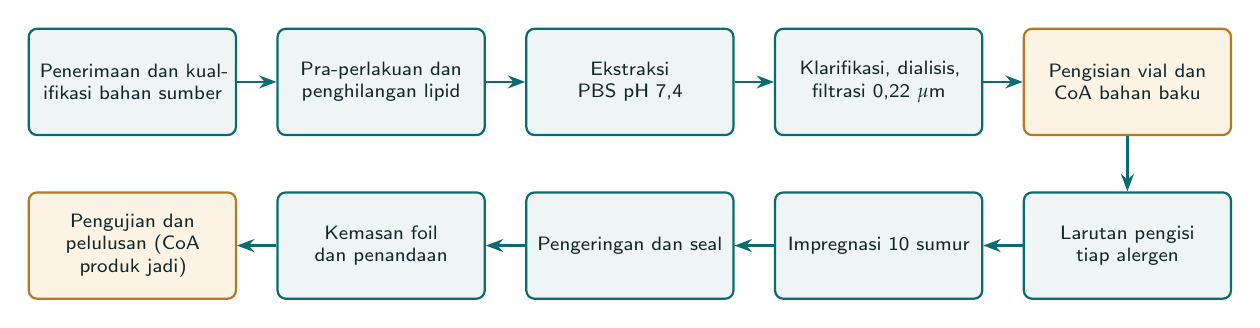
\begin{tikzpicture}[node distance=0.4cm and 0.5cm]
 \node[flow] (a) {Penerimaan dan kualifikasi bahan sumber};
 \node[flow,right=of a] (b) {Pra-perlakuan dan penghilangan lipid};
 \node[flow,right=of b] (c) {Ekstraksi PBS pH 7,4};
 \node[flow,right=of c] (d) {Klarifikasi, dialisis, filtrasi 0,22 $\mu$m};
 \node[gate,right=of d] (e) {Pengisian vial dan CoA bahan baku};
 \node[flow,below=0.7cm of e] (f) {Larutan pengisi tiap alergen};
 \node[flow,left=of f] (g) {Impregnasi 10 sumur};
 \node[flow,left=of g] (h) {Pengeringan dan seal};
 \node[flow,left=of h] (i) {Kemasan foil dan penandaan};
 \node[gate,left=of i] (j) {Pengujian dan pelulusan (CoA produk jadi)};
 \draw[arr] (a)--(b); \draw[arr] (b)--(c); \draw[arr] (c)--(d); \draw[arr] (d)--(e);
 \draw[arr] (e)--(f); \draw[arr] (f)--(g); \draw[arr] (g)--(h); \draw[arr] (h)--(i); \draw[arr] (i)--(j);
\end{tikzpicture}
\caption{Alur produksi dua tahap. Baris atas: ekstrak alergen. Baris bawah: patch.}
\label{fig:alur}
\end{figure}

\begin{table}[H]
\centering
\caption{Langkah pembuatan ekstrak, parameter, dan kendali dalam proses.}
\label{tab:t1}
{\footnotesize\tabstart\setlength{\tabcolsep}{3.5pt}
\begin{tabular}{@{}rL{2.7cm}L{6.4cm}L{4.4cm}@{}}
\toprule
\hdrrow\tH{No} & \tH{Langkah} & \tH{Parameter proses} & \tH{Kendali dalam proses} \\
\midrule
1 & Penerimaan bahan sumber & Pemeriksaan identitas, kondisi, dan dokumen pemasok; penyimpanan sesuai bahan & Kriteria Tabel~\ref{tab:sumber}, status karantina \\
2 & Pra-perlakuan & Udang: otot 500 g dipotong dan digiling. Tungau: biakan dipanen minggu ke-3. Bahan lain: dipotong, digiling, atau diayak & Bobot, waktu panen \\
3 & Penghilangan lipid dan pigmen & Aseton 1:1 (b/v), pengadukan, penyaringan & Kadar lipid (tungau), warna filtrat \\
4 & Pengeringan & Semalam di lemari asam pada 25 $^\circ$C sampai aseton menguap sempurna & Bau aseton, bobot konstan \\
5 & Ekstraksi & PBS pH 7,4, nisbah 1:10 (b/v), 25 $^\circ$C, pengadukan lembut 4 jam & pH, suhu, waktu \\
6 & Klarifikasi & Sentrifugasi 10.000 $\times g$, 20 menit, 4 $^\circ$C; filtrasi 0,45 $\mu$m & Kejernihan supernatan \\
7 & Dialisis dan pemekatan & Dialisis terhadap PBS pada 4 $^\circ$C, tiga kali ganti dalam 24 jam; pemekatan ultrafiltrasi ke 0,5 sampai 2,5 mg/mL & Protein total (Bradford) \\
8 & Filtrasi steril dan pengisian & Filtrasi 0,22 $\mu$m, pengisian 5 mL per vial dalam kabinet keamanan hayati & Volume isi, jumlah vial, integritas tutup \\
9 & Karakterisasi dan pelulusan & pH, nitrogen total, protein, SDS-PAGE, penanda alergen, aktivitas alergenik, mikrobiologi, endotoksin & Seluruh parameter CoA bahan baku \\
10 & Penyimpanan & 2 sampai 8 $^\circ$C, terlindung cahaya & Pemantauan suhu kontinu \\
\bottomrule
\end{tabular}}
\end{table}

\subsection{Ekstrak acuan internal}\label{sec:ihrp}

Ekstrak acuan internal (IHRP) tiap alergen dibuat dari satu produksi, dikarakterisasi penuh, dialikuotkan, dan disimpan pada $-20$ $^\circ$C. Aktivitas alergenik tiap batch ekstrak dinyatakan sebagai persen terhadap IHRP dengan uji inhibisi pengikatan IgE kompetitif memakai serum pool 10 sampai 15 individu atopik, dan batas penerimaan adalah 80 sampai 125\% IHRP \cite{ema}. IHRP baru dibandingkan dengan IHRP lama sebelum menggantikannya.

\Needspace{22\baselineskip}
\section{Tahap 2: pembuatan patch}

\subsection{Kebutuhan ekstrak per batch}

Larutan pengisi memakai ekstrak apa adanya tanpa pengenceran, sehingga volume isi tiap sumur ditentukan oleh kadar protein batch ekstrak: volume ($\mu$L) = 30 $\mu$g dibagi kadar protein (mg/mL). Tabel~\ref{tab:alg} menghitung kebutuhan untuk satu batch 1.000 patch dengan kelebihan isi 20\% untuk kehilangan proses dan sampel kendali.

\begin{table}[H]
\centering
\caption{Volume isi dan kebutuhan ekstrak per batch patch 1.000 buah.}
\label{tab:alg}
{\footnotesize\tabstart\setlength{\tabcolsep}{3.5pt}
\begin{tabular}{@{}L{2.9cm}L{3.2cm}R{1.8cm}R{1.8cm}R{1.9cm}R{1.2cm}R{1.5cm}@{}}
\toprule
\hdrrow\tH{Ekstrak} & \tH{Batch ekstrak} & \tH{Protein (mg/mL)} & \tH{Volume per sumur ($\mu$L)} & \tH{Volume per batch (mL)} & \tH{Vial 5 mL} & \tH{Batch patch per batch ekstrak} \\
\midrule
Tungau debu rumah & ALG-HDM-2608-01 & 1,12 & 26,8 & 32,1 & 7 & 15 \\
Udang & ALG-UDG-2608-01 & 0,86 & 34,9 & 41,9 & 9 & 11 \\
Susu sapi & ALG-SSP-2608-01 & 1,45 & 20,7 & 24,8 & 5 & 20 \\
Daging sapi & ALG-DSP-2608-01 & 1,02 & 29,4 & 35,3 & 8 & 14 \\
Daging ayam & ALG-AYM-2608-01 & 0,94 & 31,9 & 38,3 & 8 & 13 \\
Putih telur & ALG-PTL-2608-01 & 0,78 & 38,5 & 46,2 & 10 & 10 \\
Gandum & ALG-GDM-2608-01 & 1,31 & 22,9 & 27,5 & 6 & 18 \\
Kacang tanah & ALG-KCT-2608-01 & 1,88 & 16,0 & 19,1 & 4 & 26 \\
Kelapa & ALG-KLP-2608-01 & 0,64 & 46,9 & 56,2 & 12 & 8 \\
Polen rumput bermuda & ALG-PLN-2608-01 & 1,57 & 19,1 & 22,9 & 5 & 21 \\
\bottomrule
\end{tabular}}
\end{table}

\subsection{Langkah, parameter, dan kendali}

\begin{table}[H]
\centering
\caption{Langkah pembuatan patch, parameter proses, dan kendali dalam proses.}
\label{tab:t2}
{\footnotesize\tabstart\setlength{\tabcolsep}{3.5pt}
\begin{tabular}{@{}rL{2.6cm}L{6.5cm}L{4.4cm}@{}}
\toprule
\hdrrow\tH{No} & \tH{Langkah} & \tH{Parameter proses} & \tH{Kendali dalam proses} \\
\midrule
1 & Persiapan matriks dan penyangga & Lembar penyangga 20 $\times$ 50 mm, 10 disk matriks berdiameter 7 mm pada posisi sesuai gambar desain; 20 sampai 25 $^\circ$C, RH 30 sampai 50\% & Dimensi dan posisi sumur, $n = 10$ per lot \\
2 & Penyiapan larutan pengisi & Vial ekstrak diseimbangkan ke suhu ruang 30 menit, dihomogenkan perlahan, dipindah ke reservoir dispenser per alergen & Protein tiap larutan, $\pm 10\%$ dari CoA \\
3 & Impregnasi & Dispenser presisi 10 jarum, satu jarum dan satu jalur per alergen; volume 16,0 sampai 46,9 $\mu$L per sumur; 20 patch per menit & Bobot isi tiap 50 patch, $\pm 5\%$; pemeriksaan sumur tidak rata \\
4 & Pengeringan & Lemari pengering terkontrol, 30 $\pm$ 2 $^\circ$C, RH $\leq 20\%$, 4 jam & Kadar air matriks $\leq 5\%$ \\
5 & Pemasangan seal & Film seal pelindung, 110 $^\circ$C, 0,4 MPa, 1,5 detik & Keutuhan seal, tanpa kebocoran antarsumur \\
6 & Pengemasan foil & Satu patch dan satu sachet silika gel per kantong, penyegelan 140 $^\circ$C, 2 detik & Keutuhan kantong, uji kebocoran \\
7 & Penandaan dan karantina & Nomor batch, kedaluwarsa, penyimpanan; patch diberi status karantina & Rekonsiliasi label dan jumlah \\
8 & Pengujian dan pelulusan & Seluruh parameter CoA produk jadi & Keputusan oleh bagian mutu \\
\bottomrule
\end{tabular}}
\end{table}

\subsection{Pencegahan kontaminasi silang antarsumur}

Setiap alergen memakai jarum, jalur cairan, dan reservoir sendiri. Jarum tidak dipakai bergantian antaralergen, dan sisa larutan tidak digabung. Urutan pengisian ditetapkan tetap dan dicatat. Pengujian migrasi antarsumur dilakukan pada tiap batch (CoA produk jadi, nomor 10), dan pengisian dihentikan bila penanda alergen terdeteksi pada sumur tetangga.

\Needspace{22\baselineskip}
\section{Atribut mutu kritis}

\begin{table}[H]
\centering
\caption{Atribut mutu kritis patch Alergen dan pengendaliannya.}
\label{tab:caq}
{\footnotesize\tabstart\setlength{\tabcolsep}{3.5pt}
\begin{tabular}{@{}L{3.3cm}L{5.0cm}L{3.4cm}L{3.0cm}@{}}
\toprule
\hdrrow\tH{Atribut} & \tH{Mengapa kritis} & \tH{Metode} & \tH{Titik kendali} \\
\midrule
Identitas tiap ekstrak & Sumur yang salah isi membuat hasil dibaca pada alergen yang keliru & ELISA penanda, SDS-PAGE & Ekstrak dan patch \\
Protein dan alergen utama per sumur & Dosis menentukan reaksi, termasuk positif atau negatif palsu & Bradford, ELISA & Ekstrak, larutan pengisi, patch \\
Aktivitas alergenik & Kadar protein tidak menjamin aktivitas IgE \cite{ema} & Inhibisi pengikatan IgE & Ekstrak dan patch \\
Konsistensi antarbatch & Bahan alam bervariasi \cite{ema} & Perbandingan dengan IHRP & Tiap batch ekstrak \\
Kontaminasi silang & Ekstrak sumur lain dapat menimbulkan reaksi palsu & Uji migrasi antarsumur & Pengisian dan seal \\
Keutuhan seal dan kemasan & Seal melindungi ekstrak sebelum aplikasi & Visual, uji kebocoran & Seal dan kemasan \\
Mutu mikrobiologi & Patch menempel pada kulit \cite{ph514} & TAMC, TYMC, patogen tertentu & Produk jadi \\
Kestabilan & Menentukan masa simpan & Studi waktu nyata \cite{ema} & Ekstrak dan patch \\
\bottomrule
\end{tabular}}
\end{table}

\section{Fasilitas, lingkungan, dan peralatan}

\subsection{Klasifikasi area}

\begin{table}[H]
\centering
\caption{Klasifikasi area dan pemantauan lingkungan.}
\label{tab:area}
{\footnotesize\tabstart\setlength{\tabcolsep}{3.5pt}
\begin{tabular}{@{}L{4.2cm}L{2.6cm}L{4.4cm}L{3.4cm}@{}}
\toprule
\hdrrow\tH{Area} & \tH{Kelas} & \tH{Pemantauan} & \tH{Frekuensi} \\
\midrule
Penerimaan dan karantina bahan & Terkendali & Suhu, kebersihan & Harian \\
Pra-perlakuan dan ekstraksi & ISO 8 & Suhu, partikel, tekanan diferensial & Harian, partikel bulanan \\
Pengisian vial ekstrak & ISO 5 dalam kabinet, latar ISO 7 & Partikel, cawan sedimentasi, cawan kontak & Tiap batch \\
Impregnasi dan pengeringan patch & ISO 8 & Suhu, RH, partikel & Tiap batch \\
Pengemasan dan penandaan & ISO 8 & Suhu, RH & Harian \\
Penyimpanan dingin 2 sampai 8 $^\circ$C & Terpetakan & Suhu kontinu dengan alarm & Kontinu \\
\bottomrule
\end{tabular}}
\end{table}

\subsection{Daftar peralatan}

\begin{table}[H]
\centering
\caption{Peralatan utama, kalibrasi, dan kualifikasi.}
\label{tab:alat}
{\footnotesize\tabstart\setlength{\tabcolsep}{3.5pt}
\begin{tabular}{@{}L{2.2cm}L{5.4cm}L{3.8cm}L{3.2cm}@{}}
\toprule
\hdrrow\tH{Kode} & \tH{Peralatan} & \tH{Dipakai pada} & \tH{Kalibrasi} \\
\midrule
EQ-EXT-01 & Lemari asam dan oven pengering & Delipidasi, pengeringan & Tahunan \\
EQ-EXT-02 & Sentrifus berpendingin & Klarifikasi & Tahunan \\
EQ-EXT-03 & Unit dialisis dan ultrafiltrasi & Dialisis, pemekatan & Tahunan \\
EQ-EXT-04 & Kabinet keamanan hayati kelas II & Filtrasi steril, pengisian & Semesteran \\
EQ-PAT-01 & Dispenser impregnasi otomatis 10 jarum & Impregnasi & Semesteran \\
EQ-PAT-02 & Lemari pengering terkontrol RH & Pengeringan patch & Tahunan \\
EQ-PAT-03 & Mesin seal panas & Pemasangan seal & Semesteran \\
EQ-PAT-04 & Mesin penyegel foil & Pengemasan foil & Semesteran \\
EQ-QC-01 & Pembaca ELISA & Penanda, aktivitas & Tahunan \\
EQ-QC-02 & pH meter, neraca analitik & pH, bobot isi & Tiap pemakaian, tahunan \\
EQ-QC-03 & Sistem elektroforesis SDS-PAGE & Profil protein & Tahunan \\
EQ-ST-01 & Lemari pendingin 2 sampai 8 $^\circ$C dan freezer $-20$ $^\circ$C & Penyimpanan & Pemetaan tahunan \\
\bottomrule
\end{tabular}}
\end{table}

\Needspace{26\baselineskip}
\section{Catatan produksi batch (terisi)}\label{sec:bpr}

Bagian ini memuat catatan produksi satu batch patch yang telah terisi, yaitu batch ALG-P-2610-01. Seluruh nilai konsisten dengan CoA produk jadi.

\begin{table}[H]
\centering
\caption{Identitas batch.}
\label{tab:bpr0}
\tabstart
\begin{tabular}{@{}L{4.2cm}L{4.4cm}L{3.0cm}L{3.4cm}@{}}
\toprule
\hdrrow\tH{Butir} & \tH{Isi} & \tH{Butir} & \tH{Isi} \\
\midrule
No. batch & ALG-P-2610-01 & Ukuran batch & 1.000 patch \\
Tanggal produksi & 6 Oktober 2026 & Tanggal rilis & 22 Oktober 2026 \\
Dokumen induk & MPR/ALG-P/01, rev. 1 & No. catatan & BPR/ALG-P/2610/01 \\
Kedaluwarsa & Oktober 2027 & Area produksi & Suite patch, ISO 8 \\
\bottomrule
\end{tabular}
\end{table}

\subsection{Ekstrak yang dipakai}

\begin{table}[H]
\centering
\caption{Lot ekstrak yang dipakai pada batch ALG-P-2610-01.}
\label{tab:bprlot}
{\footnotesize\tabstart\setlength{\tabcolsep}{3.5pt}
\begin{tabular}{@{}rL{3.0cm}L{3.3cm}R{2.2cm}R{2.4cm}@{\hspace{14pt}}L{2.0cm}@{}}
\toprule
\hdrrow\tH{Sumur} & \tH{Ekstrak} & \tH{Lot} & \tH{Dipakai (mL)} & \tH{Dipakai, vial} & \tH{Status} \\
\midrule
1 & Tungau debu rumah & ALG-HDM-2608-01 & 28,1 & 6 & Lulus CoA \\
2 & Udang & ALG-UDG-2608-01 & 36,6 & 8 & Lulus CoA \\
3 & Susu sapi & ALG-SSP-2608-01 & 21,7 & 5 & Lulus CoA \\
4 & Daging sapi & ALG-DSP-2608-01 & 30,9 & 7 & Lulus CoA \\
5 & Daging ayam & ALG-AYM-2608-01 & 33,5 & 7 & Lulus CoA \\
6 & Putih telur & ALG-PTL-2608-01 & 40,4 & 9 & Lulus CoA \\
7 & Gandum & ALG-GDM-2608-01 & 24,0 & 5 & Lulus CoA \\
8 & Kacang tanah & ALG-KCT-2608-01 & 16,8 & 4 & Lulus CoA \\
9 & Kelapa & ALG-KLP-2608-01 & 49,2 & 10 & Lulus CoA \\
10 & Polen rumput bermuda & ALG-PLN-2608-01 & 20,1 & 5 & Lulus CoA \\
\bottomrule
\end{tabular}}
\end{table}

\subsection{Langkah proses dan hasil aktual}

\begin{table}[H]
\centering
\caption{Catatan langkah proses batch ALG-P-2610-01.}
\label{tab:bpr1}
{\footnotesize\tabstart\setlength{\tabcolsep}{3.2pt}
\begin{tabular}{@{}rL{2.5cm}L{3.5cm}L{4.0cm}L{2.5cm}@{}}
\toprule
\hdrrow\tH{No} & \tH{Langkah} & \tH{Target} & \tH{Hasil aktual} & \tH{Waktu, paraf} \\
\midrule
1 & Pemeriksaan area dan jalur & Area bersih, jalur terpisah & Sesuai, 10 jalur & 6 Okt, 08.00, Operator 1 \\
2 & Persiapan matriks & 10 disk, posisi sesuai desain & Sesuai, $n=10$ & 6 Okt, 08.30, Operator 1 \\
3 & Protein larutan pengisi & Dalam $\pm 10\%$ CoA & Selisih $-3,1$ sampai $+4,2\%$ & 6 Okt, 09.15, Analis QC \\
4 & Impregnasi & 16,0 sampai 46,9 $\mu$L, 20 patch/menit & Bobot isi $\pm 3,4\%$, 50 menit & 6 Okt, 10.00 sampai 10.50, Operator 2 \\
5 & Pengeringan & 30 $\pm$ 2 $^\circ$C, RH $\leq 20\%$, 4 jam & 30,4 $^\circ$C, RH 17\%, 4 jam & 6 Okt, 11.00 sampai 15.00, Operator 2 \\
6 & Kadar air matriks & $\leq 5\%$ & 3,6\% (rata-rata $n=10$) & 6 Okt, 15.10, Analis QC \\
7 & Pemasangan seal & 110 $^\circ$C, 0,4 MPa, 1,5 detik & 110 $^\circ$C, 0,4 MPa, 1,5 detik & 7 Okt, 08.30, Operator 3 \\
8 & Pemeriksaan seal & Tanpa kebocoran & 14 patch ditolak & 7 Okt, 10.30, Operator 3 \\
9 & Pengemasan foil & 140 $^\circ$C, 2 detik, silika gel & Sesuai & 7 Okt, 13.00, Operator 3 \\
10 & Penandaan & Batch dan kedaluwarsa benar & Rekonsiliasi label sesuai & 7 Okt, 15.00, Penyelia \\
11 & Karantina dan pengambilan sampel & Sampel uji dan pertinggal & 30 sampel uji, 20 pertinggal & 8 Okt, 09.00, Analis QC \\
12 & Pelulusan & CoA produk jadi lulus & Lulus, 22 Oktober 2026 & 22 Okt, Kepala mutu \\
\bottomrule
\end{tabular}}
\end{table}

\subsection{Rekonsiliasi dan hasil}

\begin{table}[H]
\centering
\caption{Rekonsiliasi jumlah patch batch ALG-P-2610-01.}
\label{tab:rekon}
\footnotesize\tabstart\renewcommand{\arraystretch}{1.0}
\begin{tabular}{@{}L{7.0cm}R{3.0cm}R{3.0cm}@{}}
\toprule
\hdrrow\tH{Uraian} & \tH{Jumlah} & \tH{Persen} \\
\midrule
Patch diisi dan dikeringkan & 1.000 & 100,0\% \\
Ditolak pada pemeriksaan seal & 14 & 1,4\% \\
Sampel pengujian (destruktif) & 30 & 3,0\% \\
Sampel pertinggal & 20 & 2,0\% \\
Patch lulus dan dirilis & 936 & 93,6\% \\
\bottomrule
\end{tabular}
\end{table}

Hasil akhir 93,6\% berada di atas batas tindakan 90\%. Tidak ada penyimpangan mayor; satu catatan minor (14 patch seal cacat) diselesaikan dengan menolak patch terkait dan memeriksa ulang suhu seal.

\Needspace{3\baselineskip}
\begin{tabular}{@{}p{5.1cm}p{5.1cm}p{5.1cm}@{}}
\rule{0pt}{12pt}\isi[4.5cm] & \isi[4.5cm] & \isi[4.5cm]\\
{\sffamily\scriptsize\color{muted}Kepala produksi, 22 Oktober 2026} & {\sffamily\scriptsize\color{muted}Kepala bagian mutu, 22 Oktober 2026} & {\sffamily\scriptsize\color{muted}Penanggung jawab, 22 Oktober 2026}\\
\end{tabular}

\Needspace{20\baselineskip}
\section{Kapasitas dan skala}

Target prototipe adalah batch 1.000 patch. Kebutuhan pada skala komersial ditunjukkan pada Tabel~\ref{tab:skala}, dengan satu kit sama dengan satu patch dan 30 $\mu$g protein per alergen per patch, pada tahun ke-5 (2032) menurut empat skenario kapasitas.

\begin{table}[H]
\centering
\caption{Kebutuhan protein nominal pada tahun ke-5 (2032) menurut skenario kapasitas.}
\label{tab:skala}
\tabstart
\begin{tabular}{@{}L{3.4cm}R{2.4cm}R{2.8cm}R{2.8cm}R{2.3cm}@{}}
\toprule
\hdrrow\tH{Skenario} & \tH{Patch per tahun} & \tH{Patch per hari kerja} & \tH{Protein per alergen (g)} & \tH{Batch 1.000 patch} \\
\midrule
Regional & 20.000 & 80 & 0,60 & 20 \\
Nasional terbatas & 53.500 & 214 & 1,61 & 54 \\
Nasional dasar & 133.800 & 535 & 4,01 & 134 \\
Nasional luas & 267.600 & 1.070 & 8,03 & 268 \\
\bottomrule
\end{tabular}
\end{table}

Perhitungan memakai 250 hari kerja per tahun, dan angka protein bersifat nominal (belum termasuk kelebihan isi 20\%, sampel pengujian, dan sisa karantina). Pada skenario nasional dasar, ukuran batch dinaikkan dari 1.000 ke sekitar 10.000 patch agar jumlah batch dan pengujian per tahun tetap wajar, dan impregnasi ratusan patch per hari memakai dispenser otomatis. Kebutuhan ekstrak tetap kecil: sekitar 4 g protein per alergen per tahun.

\Needspace{24\baselineskip}
\section{Kemasan, penyimpanan, dan kestabilan}\label{sec:stab}

Patch dikemas dalam kantong foil aluminium dengan silika gel dan disimpan pada 2 sampai 8 $^\circ$C. Studi kestabilan waktu nyata dan dipercepat mengacu pada ICH Q1A(R2) dan, untuk produk biologi, ICH Q5C \cite{ema,ich}. Tabel~\ref{tab:stab} memuat protokolnya. Masa simpan 12 bulan dinyatakan pada kondisi penyimpanan dan dikonfirmasi oleh data waktu nyata.

\begin{table}[H]
\centering
\caption{Protokol kestabilan produk jadi (satu batch per kondisi, 3 batch pertama).}
\label{tab:stab}
{\footnotesize\tabstart\setlength{\tabcolsep}{3.5pt}
\begin{tabular}{@{}L{3.2cm}L{4.4cm}L{7.0cm}@{}}
\toprule
\hdrrow\tH{Kondisi} & \tH{Titik waktu (bulan)} & \tH{Parameter} \\
\midrule
2 sampai 8 $^\circ$C (waktu nyata) & 0, 3, 6, 9, 12, 18, 24 & Tampilan, protein per sumur, penanda per sumur, aktivitas alergenik, migrasi antarsumur, keutuhan seal, TAMC dan TYMC \\
25 $^\circ$C, RH 60\% (dipercepat) & 0, 1, 3, 6 & Tampilan, protein per sumur, penanda, aktivitas alergenik, keutuhan seal \\
Setelah kantong dibuka (suhu ruang) & 0, 1, 4, 8 jam & Tampilan, keutuhan seal, penyerapan lembap \\
Ekstrak (2 sampai 8 $^\circ$C) & 0, 3, 6, 9, 12 & pH, protein, SDS-PAGE, penanda, aktivitas alergenik, TAMC dan TYMC \\
\bottomrule
\end{tabular}}
\end{table}

\section{Sistem mutu}

\subsection{Pengendalian perubahan dan penyimpangan}

Perubahan pada bahan sumber, parameter proses, peralatan, atau spesifikasi diajukan melalui pengendalian perubahan dan dinilai dampaknya pada atribut mutu kritis sebelum diterapkan. Penyimpangan dicatat, diklasifikasikan, dan diselidiki sesuai Tabel~\ref{tab:dev}.

\begin{table}[H]
\centering
\caption{Klasifikasi penyimpangan.}
\label{tab:dev}
{\footnotesize\tabstart\setlength{\tabcolsep}{3.5pt}
\begin{tabular}{@{}L{2.4cm}L{6.4cm}L{3.0cm}L{2.9cm}@{}}
\toprule
\hdrrow\tH{Kelas} & \tH{Contoh} & \tH{Penyelidikan} & \tH{Keputusan batch} \\
\midrule
Kritis & Identitas ekstrak keliru, kontaminasi silang, kontaminasi mikrob & 24 jam, akar masalah dan CAPA & Batch ditolak atau ditahan \\
Mayor & Parameter proses keluar batas, suhu penyimpanan keluar batas & 5 hari kerja & Ditahan sampai dinilai mutu \\
Minor & Seal cacat terisolasi, dokumen kurang paraf & 10 hari kerja & Batch diproses, patch terkait ditolak \\
\bottomrule
\end{tabular}}
\end{table}

\subsection{Dokumen mutu}

\begin{table}[H]
\centering
\caption{Struktur dokumen mutu.}
\label{tab:sop}
{\footnotesize\tabstart\setlength{\tabcolsep}{3.5pt}
\begin{tabular}{@{}L{2.8cm}L{8.2cm}L{3.8cm}@{}}
\toprule
\hdrrow\tH{Kode} & \tH{Judul} & \tH{Pemilik} \\
\midrule
MPR/ALG-E/01 & Dokumen induk produksi ekstrak alergen & Kepala produksi \\
MPR/ALG-P/01 & Dokumen induk produksi patch Alergen & Kepala produksi \\
SOP/PR/001 & Penerimaan dan kualifikasi bahan sumber & Produksi, mutu \\
SOP/PR/002 & Ekstraksi dan dialisis & Produksi \\
SOP/PR/003 & Impregnasi dan pengeringan & Produksi \\
SOP/PR/004 & Pemasangan seal dan pengemasan foil & Produksi \\
SOP/QC/001 & Uji protein, ELISA penanda, SDS-PAGE & Pengendalian mutu \\
SOP/QC/002 & Uji aktivitas alergenik terhadap IHRP & Pengendalian mutu \\
SOP/QC/003 & Uji mikrobiologi dan endotoksin & Pengendalian mutu \\
SOP/QA/001 & Pengendalian perubahan, penyimpangan, dan CAPA & Jaminan mutu \\
SOP/QA/002 & Pelulusan batch dan penarikan produk & Jaminan mutu \\
SOP/QA/003 & Pemantauan kestabilan & Jaminan mutu \\
\bottomrule
\end{tabular}}
\end{table}

\subsection{Organisasi}

Kepala produksi bertanggung jawab atas dokumen induk dan pelaksanaan proses, kepala bagian mutu atas pengujian dan pelulusan batch, dan penanggung jawab atas keputusan akhir pelulusan. Fungsi produksi dan mutu dijalankan oleh orang yang berbeda.

\begin{thebibliography}{99}
\small
\setlength{\itemsep}{2pt}
\bibitem{ema} European Medicines Agency. Guideline on allergen products: production and quality issues. EMEA/CHMP/BWP/304831/2007, 20 November 2008.
\bibitem{ph514} European Pharmacopoeia. Bab 5.1.4, Microbiological quality of non-sterile pharmaceutical preparations and substances for pharmaceutical use.
\bibitem{ich} International Council for Harmonisation. ICH Q1A(R2): Stability testing of new drug substances and products, 2003; ICH Q5C: Stability testing of biotechnological/biological products, 1995.
\bibitem{pratama23} Pratama YA, Marhaeny HD, Kasatu SM, Rohmah L, Nurhan AD, Rahmadi M, Khotib J. The optimisation and standardisation of Indonesian house dust mites allergenic extract as a desensitising agent. Pharmacy Education 2023;23(4):137-139. doi:10.46542/pe.2023.234.137139
\bibitem{marhaeny24} Marhaeny HD, Rohmah L, Pratama YA, Kasatu SM, Miatmoko A, Addimaysqi R, dkk. Shrimp allergen extract immunotherapy induces prolonged immune tolerance in a gastro-food allergy mouse model. PLoS ONE 2024;19(12):e0315312. doi:10.1371/journal.pone.0315312
\end{thebibliography}

\end{document}
